\chapter{Graph Isomorphism, Subgraph Isomorphism and Ulam's Conjecture}

Rishnak was frantically looking for Ajur as he wanted to Ajur and share with him some important concepts. Finally he found Ajur and Jura walking along the bank of a pond in the cemetery. Rishnak told Ajur that we have been talking about Graphs and some times, we label the vertices and sometimes we do not label the vertices. Rishnak told Ajur that the graph with vertices labeled is called a labeled graph and the one without labels is called unlabeled graphs. Two labeled graphs are equivalent if they are identical- all the edges have the same labels. Here are two labeled graphs that are equivalent see Figurea \ref{8g1} and \ref{8g11}. Graph see Figure \ref{8g2} is not equivalent to either Graph \ref{8g1} or \ref{8g11} ad in Graph \ref{8g2} there is no edge between vertices 4 and 5.
\begin{figure}
\begin{center}
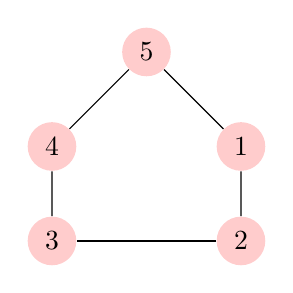
\begin{tikzpicture}
  [scale=.6,auto=left,every node/.style={circle,fill=red!20}]
  \node (n1) at (5,5) {1};
  \node (n4) at (1,5)  {4};
  \node (n3) at  (1,3) {3};
  \node (n2) at (5,3)  {2};
  \node (n5) at (3,7)  {5};

  \foreach \from/\to in {n1/n2,n2/n3,n3/n4,n4/n5,n1/n5}
    \draw (\from) -- (\to);

\end{tikzpicture}
\caption{Labeled Graph}\label{8g1}
\end{center}

\end{figure}
\begin{figure}
\begin{center}
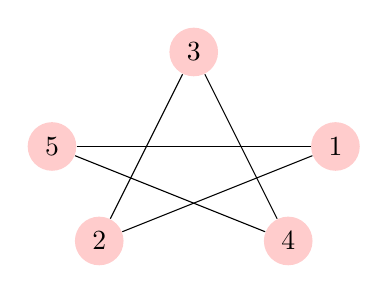
\begin{tikzpicture}
  [scale=.6,auto=left,every node/.style={circle,fill=red!20}]
   \node (n1) at (6,5) {1};
  \node (n5) at (0,5)  {5};
  \node (n2) at  (1,3) {2};
  \node (n4) at (5,3)  {4};
  \node (n3) at (3,7)  {3};

  \foreach \from/\to in {n1/n2,n2/n3,n3/n4,n4/n5,n5/n1}
    \draw (\from) -- (\to);

\end{tikzpicture}
\caption{ Another labeled graph with five vertices equivalent to Figure \ref{8g1}}\label{8g11}
\end{center}
\end{figure}

\begin{figure}
\begin{center}
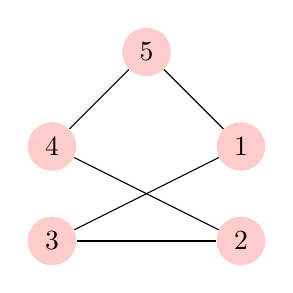
\begin{tikzpicture}
  [scale=.6,auto=left,every node/.style={circle,fill=red!20}]
   \node (n1) at (5,5) {1};
  \node (n4) at (1,5)  {4};
  \node (n3) at  (1,3) {3};
  \node (n2) at (5,3)  {2};
  \node (n5) at (3,7)  {5};


  \foreach \from/\to in {n1/n3,n2/n4,n3/n2,n1/n5,n5/n4}
    \draw (\from) -- (\to);

\end{tikzpicture}
\caption{ Another labeled graph with five vertices which is not equivalent to Graphs \ref{8g1} and \ref{8g11} as the edge labels are distinct from either of the two graphs}\label{8g2}
\end{center}
\end{figure}

Two graphs are isomorphic (structurally the same), if they are equivalent under vertex relabeling. So if in Graph \ref{8g2} vertex 2 is relabeled as 3 and vertex 3 is relabeled as 2, the two graphs \ref{8g2} and \ref{8g1} are equivalent. If a graph,$G$, is equivalent to a graph $H$ and $H$ is equivalent to another graph $P$, then $G$ is equivalent to graph $P$\footnote{Equivalence relation is transitive.}. To test whether two graphs are isomorphic are not is a hard\footnote{Not as hard as finding a Hamiltonian Cycle in a graph} problem.

if two graphs are isomorphic, they should have the same number of vertices, same number of edges, same degree sequences, length of the longest cycle, length of the shortest cycle and many more properties.  These properties of graphs are called invariant of graphs. By no mean these invariants are exhaustive. We do not know of a single invariant (that could be easily computed) that can be used to test whether or not given two  graphs are isomorphic. 

Rishnak asked Ajur, can you provide two graphs which have the same number of vertices and same number of edges but they are not isomorphic. Ajur thought a bit, and he was able to produce the following two graphs which have 6 vertices and 9 edges. Ajur added that one graph is bipartite (all cycles are of even length) \ref{8g3} and the other one is not bipartite (cycle of length 3) \ref{8g4} and hence these two graphs are not isomorphic.

\begin{figure}

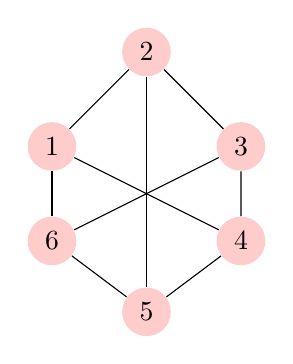
\begin{tikzpicture}
  [scale=.3,auto=left,every node/.style={circle,fill=red!20}]
  \node (n1) at (1,7) {1};
  \node (n2) at (5,11)  {2};
  \node (n3) at (9,7)  {3};
  \node (n4) at (9,3) {4};
  \node (n5) at (5,0)  {5};
  \node (n6) at (1,3) {6};
  
   \foreach \from/\to in {n1/n2,n2/n3,n3/n4,n4/n5,n5/n6,n1/n6,
  n2/n5, n6/n3,n1/n4}
    \draw (\from) -- (\to);
    \end{tikzpicture}
\caption{ A Bipartite Graph with 6 vertices and 9 edges same as Graph in \ref{5g5}}\label{8g3}

\end{figure}

\begin{figure}

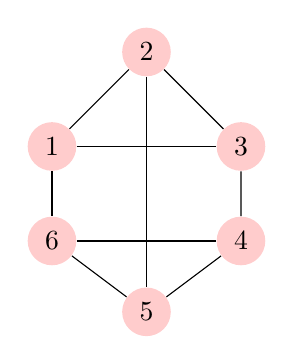
\begin{tikzpicture}
  [scale=.3,auto=left,every node/.style={circle,fill=red!20}]
  \node (n1) at (1,7) {1};
  \node (n2) at (5,11)  {2};
  \node (n3) at (9,7)  {3};
  \node (n4) at (9,3) {4};
  \node (n5) at (5,0)  {5};
  \node (n6) at (1,3) {6};
  
   \foreach \from/\to in {n1/n2,n2/n3,n3/n4,n4/n5,n5/n6,n1/n6,
  n2/n5, n6/n4,n1/n3}
    \draw (\from) -- (\to);
    \end{tikzpicture}
\caption{ A nonBipartite Graph with 6 vertices and 9 edges}\label{8g4}

\end{figure}